\documentclass[a4paper]{article}
%\usepackage[top=0, bottom=0, left=0, right=0]{geometry}
\usepackage[utf8]{inputenc}
\usepackage[english]{babel}
\usepackage{verbatim}
\usepackage{array}
\def\pdfshellescape{1}
\usepackage{epstopdf}
%\usepackage{amsmath}%massa trevliga symboler
\usepackage{graphicx}%[pdftex]
\usepackage[all]{xy}
\usepackage{mathtools}
\usepackage{listings}
\xyoption{frame}
%% Test
\usepackage{ifxetex,ifluatex}
\usepackage{etoolbox}
\usepackage[svgnames]{xcolor}
\usepackage{wrapfig}


\usepackage{tikz}

\usepackage{framed}
\usepackage{float}

\definecolor{mygreen}{rgb}{0,0.6,0}
\definecolor{mygray}{rgb}{0.5,0.5,0.5}
\definecolor{mymauve}{rgb}{0.58,0,0.82}
\lstset{   backgroundcolor=\color{white},   % choose the background color; you must add \usepackage{color} or \usepackage{xcolor}
  %basicstyle=\footnotesize,        % the size of the fonts that are used for the code
  breakatwhitespace=false,         % sets if automatic breaks should only happen at whitespace
  breaklines=true,                 % sets automatic line breaking
  %captionpos=b,                    % sets the caption-position to bottom
  commentstyle=\color{mygreen},    % comment style
  deletekeywords={...},            % if you want to delete keywords from the given language
  escapeinside={\%*}{*)},          % if you want to add LaTeX within your code
  extendedchars=true,              % lets you use non-ASCII characters; for 8-bits encodings only, does not work with UTF-8
  keepspaces=true,                 
  keywordstyle=\color{blue},       % keyword style
  language=MatLab,                 % the language of the code
  numbers=left,                    
  numbersep=5pt,                   % how far the line-numbers are from the code
  numberstyle=\tiny\color{mygray}, % the style that is used for the line-numbers
  rulecolor=\color{black},         
  showspaces=false,                
  showstringspaces=false,          % underline spaces within strings only
  showtabs=false,                  % show tabs within strings adding particular underscores
  stringstyle=\color{mymauve},     % string literal style
  tabsize=2,                       % sets default tabsize to 2 spaces
  title=\lstname
}

% conditional for xetex or luatex
\newif\ifxetexorluatex
\ifxetex
  \xetexorluatextrue
\else
  \ifluatex
    \xetexorluatextrue
  \else
    \xetexorluatexfalse
  \fi
\fi
%
\ifxetexorluatex%
  \usepackage{fontspec}
  \usepackage{libertine} % or use \setmainfont to choose any font on your system
  \newfontfamily\quotefont[Ligatures=TeX]{Linux Libertine O} % selects Libertine as the quote font
\else
  \usepackage[utf8]{inputenc}
  \usepackage[T1]{fontenc}
  \usepackage{libertine} % or any other font package
  \newcommand*\quotefont{\fontfamily{LinuxLibertineT-LF}} % selects Libertine as the quote font
\fi

\newcommand*\quotesize{60} % if quote size changes, need a way to make shifts relative
% Make commands for the quotes
\newcommand*{\openquote}
   {\tikz[remember picture,overlay,xshift=-4ex,yshift=-2.5ex]
   \node (OQ) {\quotefont\fontsize{\quotesize}{\quotesize}\selectfont``};\kern0pt}

\newcommand*{\closequote}[1]
  {\tikz[remember picture,overlay,xshift=4ex,yshift={#1}]
   \node (CQ) {\quotefont\fontsize{\quotesize}{\quotesize}\selectfont''};}

% select a colour for the shading
\colorlet{shadecolor}{Azure}

\newcommand*\shadedauthorformat{\emph} % define format for the author argument

% Now a command to allow left, right and centre alignment of the author
\newcommand*\authoralign[1]{%
  \if#1l
    \def\authorfill{}\def\quotefill{\hfill}
  \else
    \if#1r
      \def\authorfill{\hfill}\def\quotefill{}
    \else
      \if#1c
        \gdef\authorfill{\hfill}\def\quotefill{\hfill}
      \else\typeout{Invalid option}
      \fi
    \fi
  \fi}
% wrap everything in its own environment which takes one argument (author) and one optional argument
% specifying the alignment [l, r or c]
%
\newenvironment{shadequote}[2][l]%
{\authoralign{#1}
\ifblank{#2}
   {\def\shadequoteauthor{}\def\yshift{-2ex}\def\quotefill{\hfill}}
   {\def\shadequoteauthor{\par\authorfill\shadedauthorformat{#2}}\def\yshift{2ex}}
\begin{snugshade}\begin{quote}\openquote}
{\shadequoteauthor\quotefill\closequote{\yshift}\end{quote}\end{snugshade}}

%%end test

\newcommand{\HRule}{\rule{\linewidth}{0.5mm}}

\title{}

\author{Robert Stigsson -- 910814-4719, \\Fredrik Ek -- 901109-0959, \\Martin Kastebo -- 930309-3372, \\Michael Tran -- 931016-1576}

\date{\today}


\begin{document}

\begin{titlepage}

\begin{center}


% Upper part of the page 

\textsc{\LARGE Web-applications}\\[1.5cm]




% Title
\HRule \\[0.4cm]
{ \huge \bfseries Project Documentation DIT126}\\
\HRule \\[0.5cm]

\textsc{\Large DrinkApp}\\[0.4cm]

% Author and supervisor

\begin{minipage}{0.4\textwidth}
\begin{flushleft} \large
%\emph{Deltagare:}\\
Robert \textsc{Stigsson}\\
robsti@student.chalmers.se\\[0.4cm]
Fredrik \textsc{Ek}\\
ekfr@student.chalmers.se
Martin \textsc{Kastebo}\\
kastebo@student.chalmers.se
Michael \textsc{Tran}\\
gustranmi@student.gu.se

\end{flushleft}
\end{minipage}
\begin{minipage}{0.4\textwidth}
\begin{flushright} \large
\emph{} \\
910814-4719, \textsc{D}\\[0.8cm]
901109-0959, \textsc{D}\\[0.8cm]
930309-3372, \textsc{D}\\[0.8cm]
931016-1576, \textsc{GU}\\[0.8cm]


\end{flushright}
\end{minipage}\\[2.0cm]
Group 12
\vfill

% Bottom of the page
{\large \today}

\end{center}

\end{titlepage}

\tableofcontents

\pagebreak

\section{The Application}
We decided to make a drink application called DrinkApp. The app is intended for amusement and as help for making and managing drinks. It could be used in most areas. It could be used by bartenders as well the average guy/girl with an interest in making drinks. \\
\\
The application is supposed to store drinks added by different users. Combining this with a rating system will make it possible to have several different options of the same drink, where you from the rating can know which one is probably the best choice. You are also supposed to be able to add drinks to your personal favourites, so that you easily can remember which ones you wanted to try when the weekend comes.\\
\\
The main attraction should however be the drinksearch functionality where you are supposed to be able to browse for drinks by submitting either name, ingredients or both. This means that you could easily add all the drinkingredients you have at home and the application will show what drinks contain those specific ingredients. It can be anything from fruit to spices to liquor etc.

\section{User roles}
Our plan was to make it possible for an admin to edit and remove not only his own drinks, but everyone elses as well. We did however only prepare this functionality rather than finnishing it due to lack of time and other priorities.

\section{Use Cases}

\subsection{Main Page}

\begin{itemize}
\item Search for drinks by name
\item Search for drinks by ingredients
\item Search for drinks by name and ingredient
\end{itemize}

\subsection{Authenticated user}

\begin{itemize}
\item Register account
\item Log In
\item Change password/email under profile
\item Add Drinks to the database with name, ingredients, types, steps och comment
\item Watch your drinks under My Drinks
\item Enter a Drinks page to share it with your friends on example facebook using the url (Dont need to be logged in to see a drinks page)
\item Edit your own Drinks under My Drinks
\item Delete your own Drinks under My drink
\item Add drinks to My Favourite Drinks by pressing the heart button next to the drinkname while browsing for drinks
\item Watch your favourite drinks under My Favourite Drinks
\item Unfavourite your added drinks
\item Rate Drinks
\item Validation in all forms
\item Log Out
\item Log in with wrong password - fail
\end{itemize}

\subsection{Misc}

\begin{itemize}
\item All passwords are hashed and salted, BCrypt.
\item Extendted protection against SQL-, HTML-, JavaScript-, XSS- based attacks
\end{itemize}

\section{Selected approach}
We selected a component- based approach using the JSF framework.

\section{Tiers}
Our application concists of several tiers or layers
From top to bottom we have:

\subsection{Web Pages (xhtml)}
All web pages. The front-end of our application. The only parts that a user will interact with.
\subsection{BackingBeans (Java)}
All Beans that handels the functionality of the different parts of the application. Works like a minor back-end for each web page, managing all temporary data.
\subsection{Controllers (Java)}
All Controllers that handels communication between the application front-end and the database.
\subsection{ORMs (Java)}
The Object Relational Mapper where we all models are implemented in Java and translated to the underlying tier in SQL. 
\subsection{Database (SQL)}
The underlying database where are data from the application are being stored.
\subsection{Other}
Aside from these we are using css and javascript for the layout on the web pages and BCrypt as encryption algorithm for passwords. 

\section{Code Structure}
We divided our different code parts into sections looking a bit like the tiers, but with some differences.

\subsection{nu.drinkapp.auth}
Package containing classes involved in the authentication process.

\subsection{nu.drinkapp.bb}
Package containing all backing beans.

\subsection{nu.drinkapp.core}
Package containing all the core classes of the application such as the Models and their relations and helpclasses.

\subsection{nu.drinkapp.ctrl}
Package containing all controllers.

\subsection{nu.drinkapp.persistence}
Package containing all classes involved for persistence in the application.

\subsection{nu.drinkapp.wrappers}
Package containing all wrapper classes and interfaces.

\section{Other}
There are alot of things we wanted to do from the start that we simply didnt have time to finnish, and there are some things we tried to do but didnt succeed with. Here follows some:

\subsection{Functionality we tried to do without succeeding}

\subsubsection{Security}
We wanted to make the application protected against SQL,javascript and HTML-injections, something that we learned would be established by using only namedqueries or prepared statements. This succeeded for almost all queries in the project, not for all however. We tried to ask for help during the supervision hours without success. It might be because of the use of subqueries in one of the queries or something like that. Neither did we manage to get cascade to work for entities, meaning that we had to make a native delete query that first deletes from all entities, using the one we want to delete from, as a foreign key. \\
\\
This might not be a course in security, but we wanted to say that we did think of it.
As an addition, because of this, we made a function to sanitize all database inputs from the use of special characters. There are too good ways of performing injections nowadays though, so it wouldnt help versus a good hacker.

\subsubsection{Tests}
We tested our application on the go as soon as we implemented new functionality. But we also intended to make tests that could be run to easily verify that everything are working as intended. This is however something we spent countless hours trying to get to work. We tried to ask several supervisors for help without getting a proper answer. We simply dont have any more time to put into it, being the major reason to why our project doesnt contain any unit tests etc. Writing the actualy tests would would take us no time at all, but seeing as we couldnt run them it seems rather pointless at this stage.

\subsection{Ajax problems}
Something else we couldnt get to work and that the supervisors couldnt help us with was when using JSFs built-in ajax functionality the last letter in a textfield wont update with ajax.
This can be seen when using find drinks. For instance when typing something in the search field and then erasing it, it wont update in the target. We do not know why and we couldnt get help fixing it, but we are aware of it.

\subsection{Functionality we wanted to do, but didnt have time for}
Here follows some examples of functionality we didnt have time to implement:
\begin{itemize}
\item Complete an admin interface so that it would be possible for admins to edit and remove all drinks in the database no matter which user added them.
\item Add a table under myprofile with some fun facts such as how many drinks the actual user added, how the actual users drinks are rated, how many drinks the actual user have rated etc
\item Add a guestbook where users could write and suggest updated functionality etc
\item Live-feed on the home-page, that gets updated automatically when new drinks are added to the database.
\item Some kind of chat, so that users can chat with each other.
\item Facebook connectivity. So people could sign up on the application using their facebook id rather than registering on the page.
\end{itemize}

We also discussed alot of other things. Such as adding small infobuttons on all views containing forms etc. \\
\\
We are however very happy with the application as a whole. We did spend alot of time on it and belive that the result is really good. The application can be found at drinkapp.nu:8080/DrinkApp

\section{Appendix}
\subsection{UML}

\begin{figure}[H]
  \begin{center}
    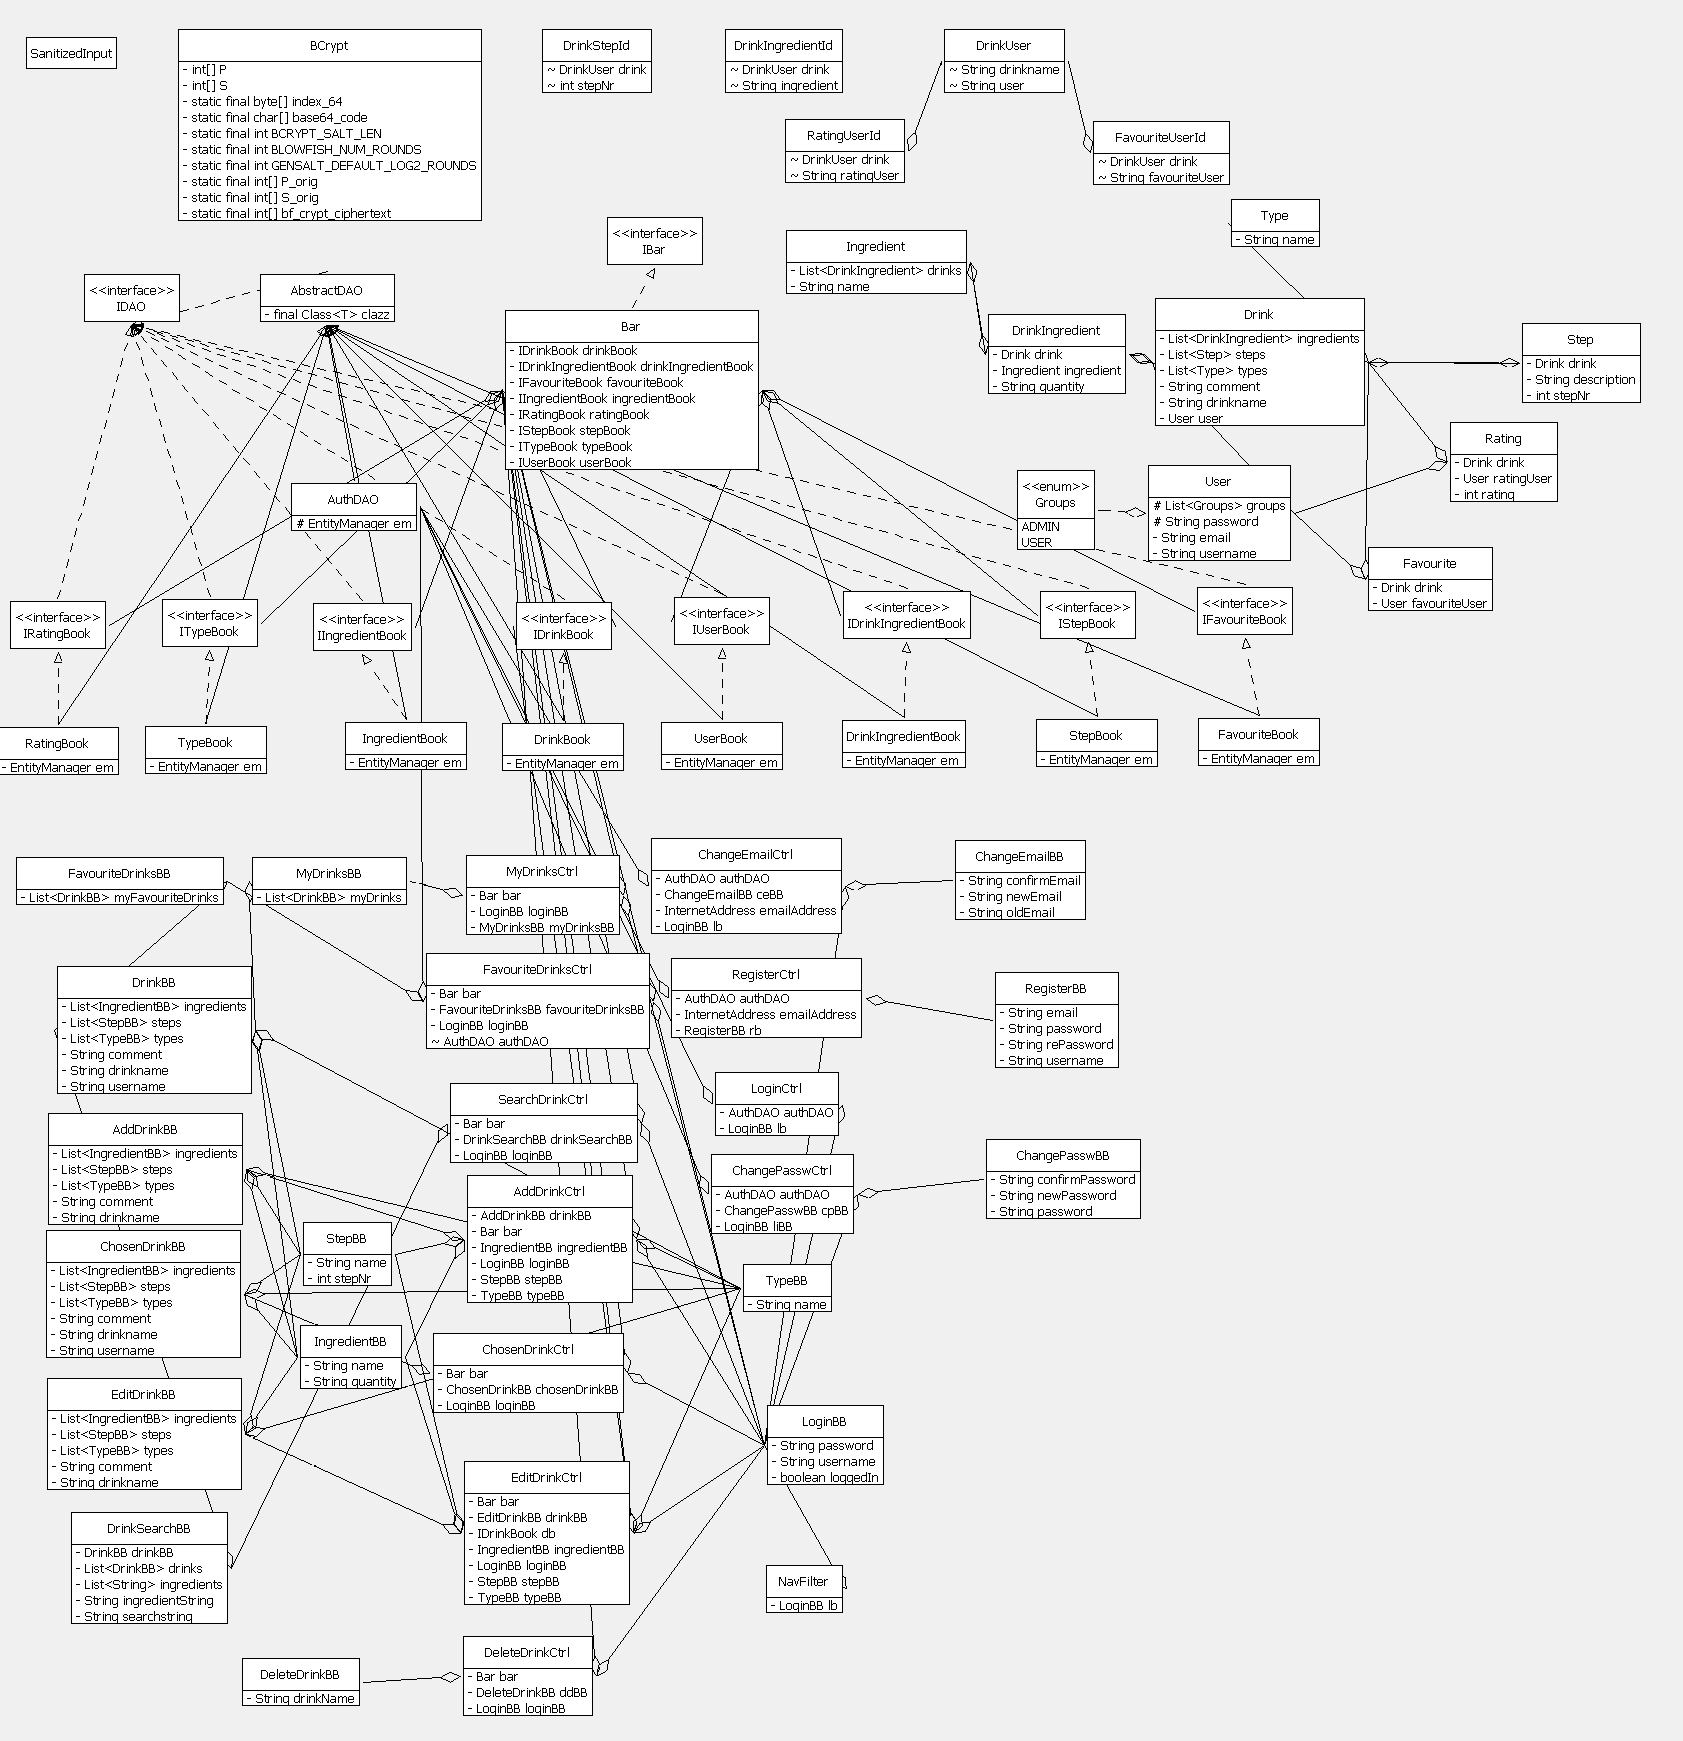
\includegraphics[width=1.3 \textwidth]{UML_final.png}
  \end{center}
  \caption{A nice UML-diagram of the application }
  \label{fig:awesomepicture}
\end{figure}

\end{document}
